\chapter{Proposed Solution}
\section{Proposed Solution}
\begin{figure}[h]
\centering
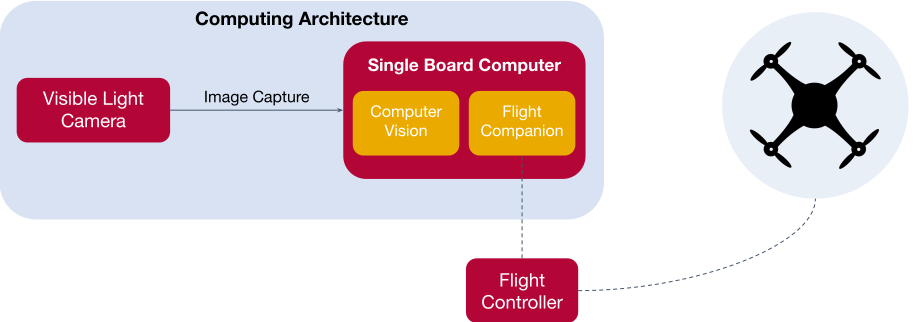
\includegraphics[width=1\linewidth]{assets/proposed-solution.png}
\caption{Proposed Solution}
\label{proposed_solution}
\end{figure}
\subsection{Hardware}
\paragraph{Single Board Computer} Nvidia Jetson Nano - 4 GB

A single board computer was imperative to achieve the non-functional design requirements outlined in~\ref{requirements}, because of their low cost, energy efficiency, size and modularity. After researching performance metrics for single board computers (SBCs) across a variety of indsutry standard computer vision models, it was determined that the NVidia Jetson Nano would be the most cost-effective and performant SBC choice, especially compared to competing platforms. On one hand, the Raspberry Pi series of SBCs would be satisfactory in regard to power usage, but significantly underpowered for computer vision applications. On the other hand, the Google Coral TPU Dev Board boasted incredible inference speeds where comparison was possible, but its major caveat consisted of only being capable of running Tensor Flow Lite (TFLite) models, which would have a significant detriment on the modularity and flexibility of the overall platform.

\paragraph{UAV Frame} HolyBro S500v2 Kit

In order to achieve the requirements of competitive flight time (compared to enterprise solutions), an accessible pricepoint, and a suitable size to mount all components, the choice was quickly narrowed down to a \textit{quadcopter}, meaning a UAV with four propellers. A quadcopter is useful for this use-case because...

\paragraph{Flight Controller} PixHawk 4

The flight controller acts as the textit{brain} of a UAV system. The PixHawk 4 was chosen because it satisfies three primary requirements of this project's design:
\begin{itemize}
\item {Autonomous flight}
\item {Detailed logging}
\item {Interface to companion computer}
\end{itemize}

\subsection{Software}
\paragraph{Flight Software} QGroundControl

QGroundControl boasts a high degree of compatibility with leading consumer and enterprise-level drone systems, including the HolyBro S500 and PixHawk 4 platform we chose for this project.
\begin{itemize}
    \item {Various route-planning tools}
    \item {Universal compatibility}
    \item {Open-souce software}
\end{itemize}

\subsection{Developer Tools}
\paragraph{JetPack Software Development Kit}

Includes:
\begin{itemize}
    \item {Jetson Linux Driver Package (L4T)}
    \item {Ubuntu 18.04 LTS Build}
    \item {CUDA accelerated libraries and APIs}
    \item {Samples, documentation and developer tools}
\end{itemize}

\paragraph{NGC Catalog} Package Manager

Easy access to AI building blocks
\begin{itemize}
    \item {Models}
    \item {Containers}
    \item {SDKs}
\end{itemize}
